\documentclass[12pt]{article}

\usepackage{fancyhdr}
\usepackage{extramarks}
\usepackage{amsmath}
\usepackage{amsthm}
\usepackage{amsfonts}
\usepackage{amssymb}
\usepackage{tikz}
\usepackage{setspace}
\usepackage{graphicx}
\usepackage[plain]{algorithm}
\usepackage{algpseudocode}
\usepackage{listings}
% \usepackage[latte,styleAll]{catppuccinpalette}
\usepackage{url}
\usetikzlibrary{automata,positioning}
\usepackage{hyperref}

%
% Basic Document Settings
%

\topmargin=-0.45in
\evensidemargin=0in
\oddsidemargin=0in
\textwidth=6.5in
\textheight=9.0in
\headsep=0.25in

\linespread{1.1}
\doublespacing

\pagestyle{fancy}
\lhead{\hmwkAuthorName}
\chead{\hmwkTitle}
\rhead{\firstxmark}
\lfoot{\lastxmark}
\cfoot{\thepage}

\setlength{\headheight}{14.5pt}
\renewcommand\headrulewidth{0.4pt}
\renewcommand\footrulewidth{0.4pt}

\setlength\parindent{0pt}

%
% Title Page
%

\title{
	\vspace{2in}
	\textmd{\textbf{\hmwkClass:\ \hmwkTitle}}\\
	\normalsize\vspace{0.1in}\small{Due\ on\ \hmwkDueDate\ at \hmwkDueTime}\\
	\vspace{0.1in}\large{\textit{\hmwkClassInstructor,\ \hmwkClassTime}}
	\vspace{3in}
}

\author{\textbf{\hmwkAuthorName}}
\date{\hmwkCompletionDate}

%
% Homework Details
%   - Title
%   - Due date
%   - Due time
%   - Course
%   - Section/Time
%   - Instructor
%   - Author
%

\newcommand{\hmwkTitle}{Final Paper - Neighborhood Tour}
\newcommand{\hmwkDueDate}{December 15, 2024}
\newcommand{\hmwkDueTime}{11:59 PM}
\newcommand{\hmwkClass}{HISP 200}
\newcommand{\hmwkClassTime}{0101}
\newcommand{\hmwkClassInstructor}{Dr. Stephan Woehlke}
\newcommand{\hmwkAuthorName}{\textbf{Vai Srivastava}}
\newcommand{\hmwkCompletionDate}{December 14, 2024}

\begin{document}

\maketitle

\pagebreak

\doublespacing

\textbf{\Large A Tour of the Evergreen Neighborhood in San Jose, California}

\section{Introduction}

Evergreen, a diverse neighborhood in East San Jose, California, embodies layers of history woven into its suburban landscape. Once part of the famed “Valley of Heart’s Delight,” the area transformed from rolling orchards and ranches into a mosaic of suburban tracts, educational institutions, and religious centers. The story of Evergreen is not only about economic expansion and demographic shifts but also about work, labor, health, and safety. Historically, Mexican and Filipino agricultural laborers harvested fruits in local orchards, while facing low wages, grueling working conditions, and exposure to hazardous pesticides. Over time, these orchards gave way to urban development and new forms of labor—service jobs in retail, educational careers, high-tech industries—many now filled by immigrants from Latin America, South and East Asia, and beyond.

In this tour, we will visit six sites that each tell a chapter in Evergreen’s larger narrative. We will explore how labor conditions have changed, how communities formed cultural and religious institutions to find safety and solidarity, how educational centers foster health and upward mobility, and how public green spaces reconnect us with the land’s farming past. By looking closely at these places, we can understand how larger global forces—immigration, industrialization, and social movements—have shaped Evergreen’s local reality. The tour will challenge you to see that the histories of work, health, and safety are living stories that continue to unfold in this community today.

\begin{figure}[h]
  \centering
  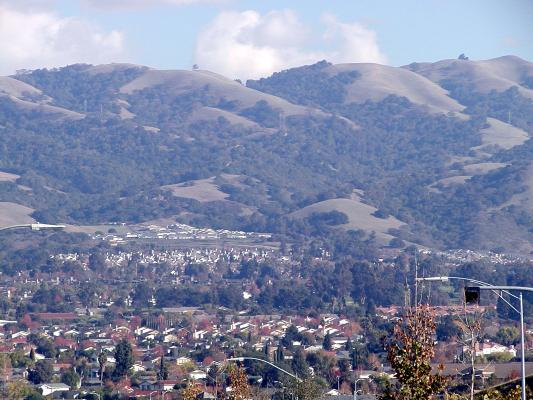
\includegraphics[width=0.8\textwidth]{assets/evergreen_landscape.png}
  \caption{San Jose's Evergreen Neighborhood}
  \label{fig:evergreen_landscape}
  \cite{eisenberg2011san}
\end{figure}

\section{Tour}

\subsection{Montgomery Hill Park}

Montgomery Hill Park, perched on gentle slopes in Evergreen, offers a view that once encompassed a rich patchwork of orchards and farmland. In the early 20th century, this land was the workplace for migrant laborers who painstakingly tended fruit trees under the hot California sun. Mexican and Filipino agricultural workers, often living in crowded and substandard conditions, were vital to the regional economy but seldom reaped the benefits of their labor \cite{pitti2018the}. Their stories reflect larger national patterns of labor exploitation and shifting immigration policies that allowed agribusiness to thrive while leaving workers vulnerable.

Today, the park’s open fields and walking trails symbolize the dramatic economic and social shifts of the area. From here, visitors can contemplate how generations of laborers—often marginalized and overlooked—helped shape Evergreen’s identity, forging a community that could later advocate for better working conditions and equal rights.

\begin{figure}[h]
  \centering
  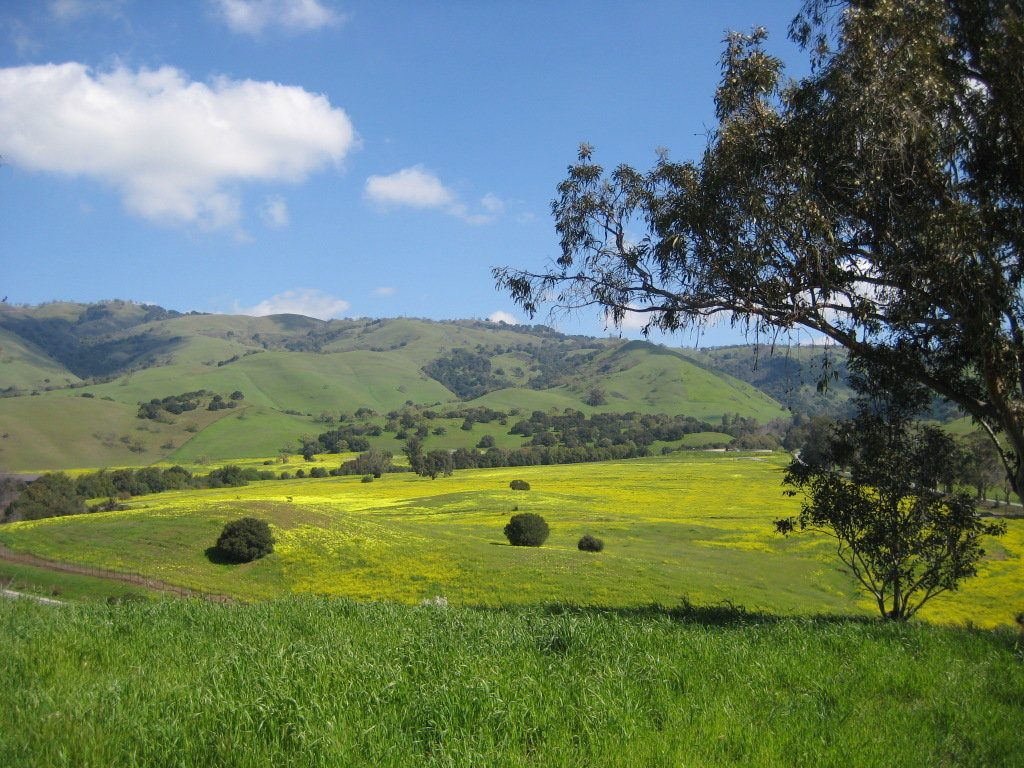
\includegraphics[width=0.8\textwidth]{assets/montgomery_hill.png}
  \caption{Montgomery Hill Park in San Jose}
  \label{fig:montgomery_hill}
  \cite{a2017montgomery}
\end{figure}

\subsection{Sikh Gurdwara San Jose}

The Sikh Gurdwara on Murillo Avenue, one of the largest in North America, represents more than just a religious institution. Founded and maintained by a thriving South Asian immigrant community, it serves as a safe, inclusive space where individuals can find spiritual, emotional, and communal nourishment. Here, the concepts of health and safety extend beyond the physical, embracing mental well-being and cultural continuity.

Amid changing labor markets—where immigrants have found work in everything from tech to transportation—this Gurdwara provides essential support. Facing language barriers, discrimination, and the stressors of low-wage work, community members gather here for free meals (langar), healthcare screenings, and legal workshops addressing workers’ rights. The Gurdwara’s story shows how religious and cultural institutions can respond to larger structural inequalities, offering solidarity and empowerment to those navigating the complex intersections of race, labor, and health in American society.

\begin{figure}[h]
  \centering
  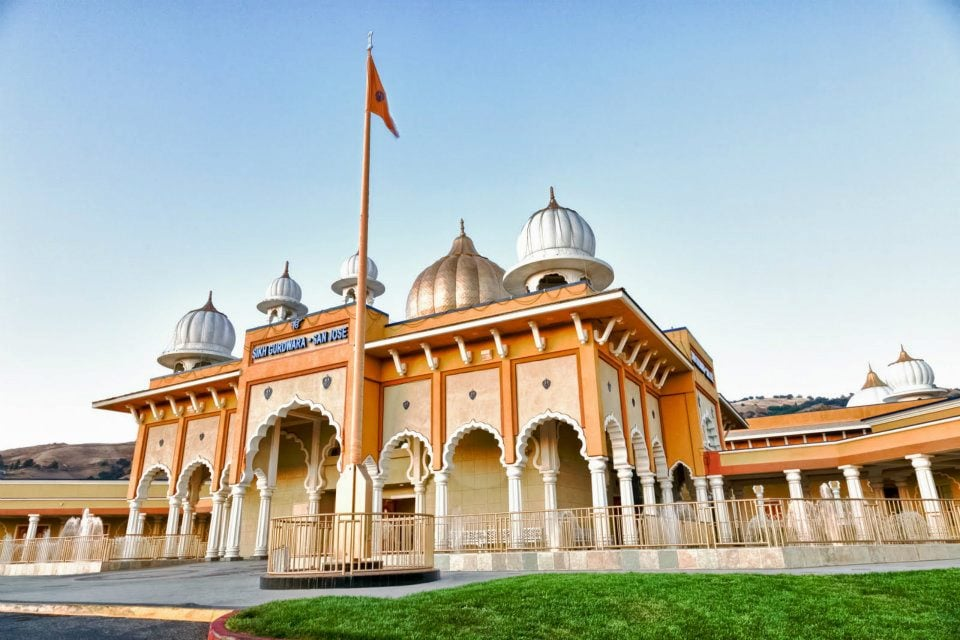
\includegraphics[width=0.8\textwidth]{assets/sikh_gurdwara.png}
  \caption{Sikh Gurdwara Sahib in San Jose}
  \label{fig:sikh_gurdwara}
  \cite{a2017sikh}
\end{figure}

\subsection{Evergreen Village Square}

Evergreen Village Square is a modern suburban plaza that stands in stark contrast to the agricultural past. Alongside cafés, retail shops, and a community library, this square represents the evolution of labor from seasonal fieldwork to stable, service-oriented employment. Yet, these service jobs—often held by women, immigrants, and people of color—still raise questions about wages, job security, and safe working conditions.

As the orchards vanished, new industries arrived, including high-tech firms and service economies. Some residents have found upward mobility through education and entrepreneurship, while others remain in low-paying jobs without benefits or protections, reflecting national trends in labor stratification \cite{cohen2011braceros}. At Evergreen Village Square, you can observe the interplay of old and new labor systems. Beyond the pleasant façade of suburban life, the plaza invites you to consider who does the work behind each product and service you enjoy.

\begin{figure}[h]
  \centering
  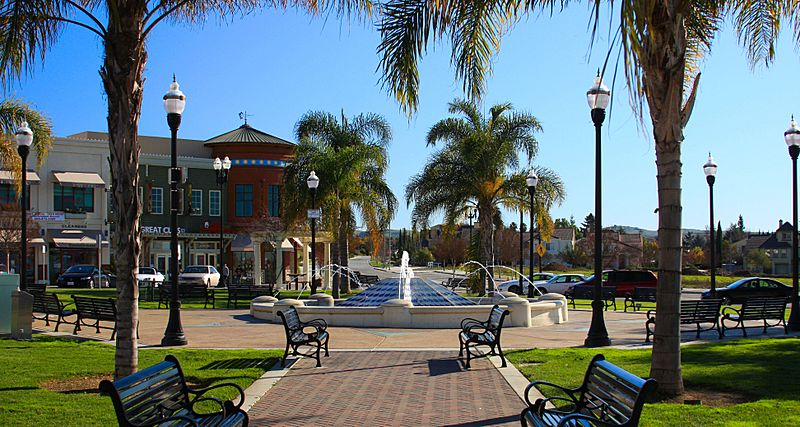
\includegraphics[width=0.8\textwidth]{assets/village_square.png}
  \caption{Evergreen Village Square in San Jose}
  \label{fig:village_square}
  \cite{thetahoeguyevergreen}
\end{figure}

\subsection{Evergreen Valley College}

Evergreen Valley College (EVC) is more than an educational institution; it’s a critical site for community health and safety. Through accessible higher education, job training, and health-related programs, EVC addresses some of the root causes of economic precarity and public health disparities. Students here come from diverse backgrounds—Vietnamese, Mexican, Indian, Filipino, African American—reflecting Evergreen’s multicultural character.

EVC’s nursing and health sciences programs train future caregivers who will serve local clinics and hospitals, bridging gaps in cultural competency and language. Workshops on worker rights, mental health support groups, and public safety initiatives empower both students and surrounding communities. At EVC, education becomes a tool not only for professional advancement but for fostering safer, healthier communities. Its role underscores how institutions can challenge systemic inequalities, placing health, self-determination, and collective well-being at the center of community development.

\begin{figure}[h]
  \centering
  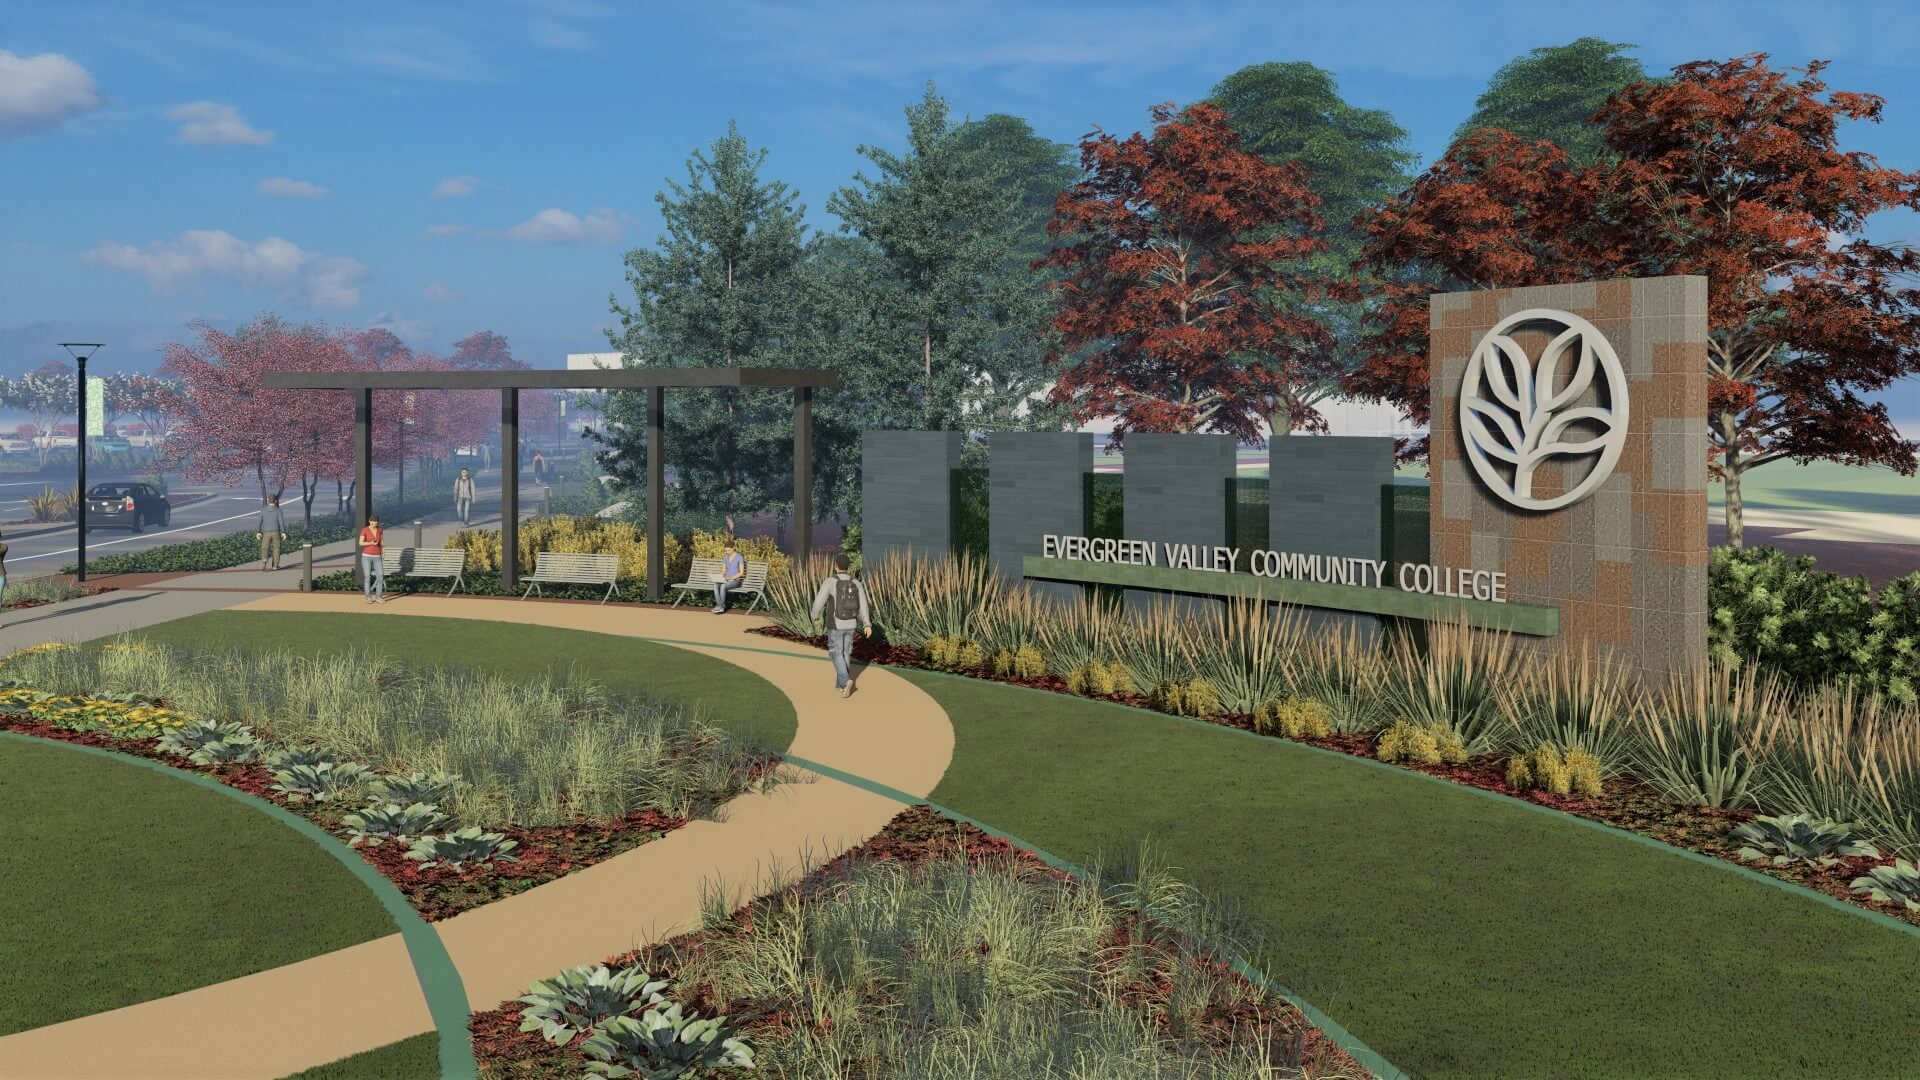
\includegraphics[width=0.8\textwidth]{assets/evc_entry.png}
  \caption{Evergreen Valley College in San Jose}
  \label{fig:evc_entry}
  \cite{a2014sjeccd}
\end{figure}

\subsection{Emma Prusch Farm Park}

Although slightly west of Evergreen’s official boundaries, Emma Prusch Farm Park remains a vital reminder of the region’s agricultural roots. Once farmland similar to Evergreen’s lost orchards, it now serves as a living museum of Santa Clara Valley’s agrarian heritage. Visitors encounter heritage fruit trees and displays that recall the intense manual labor required to sustain orchard economies.

Historically, these fields were sites of both opportunity and exploitation. Agricultural workers—often recruited through the Bracero Program or arriving as refugees—battled long hours, chemical hazards, and uncertain contracts \cite{cohen2011braceros, pitti2018the}. Emma Prusch Farm Park encourages visitors to consider how past labor struggles shape present conversations about fair wages and safe working environments. Standing amidst the carefully maintained greenery, one can appreciate the longstanding human effort that once sustained an economy and question how we value labor today.

\begin{figure}[h]
  \centering
  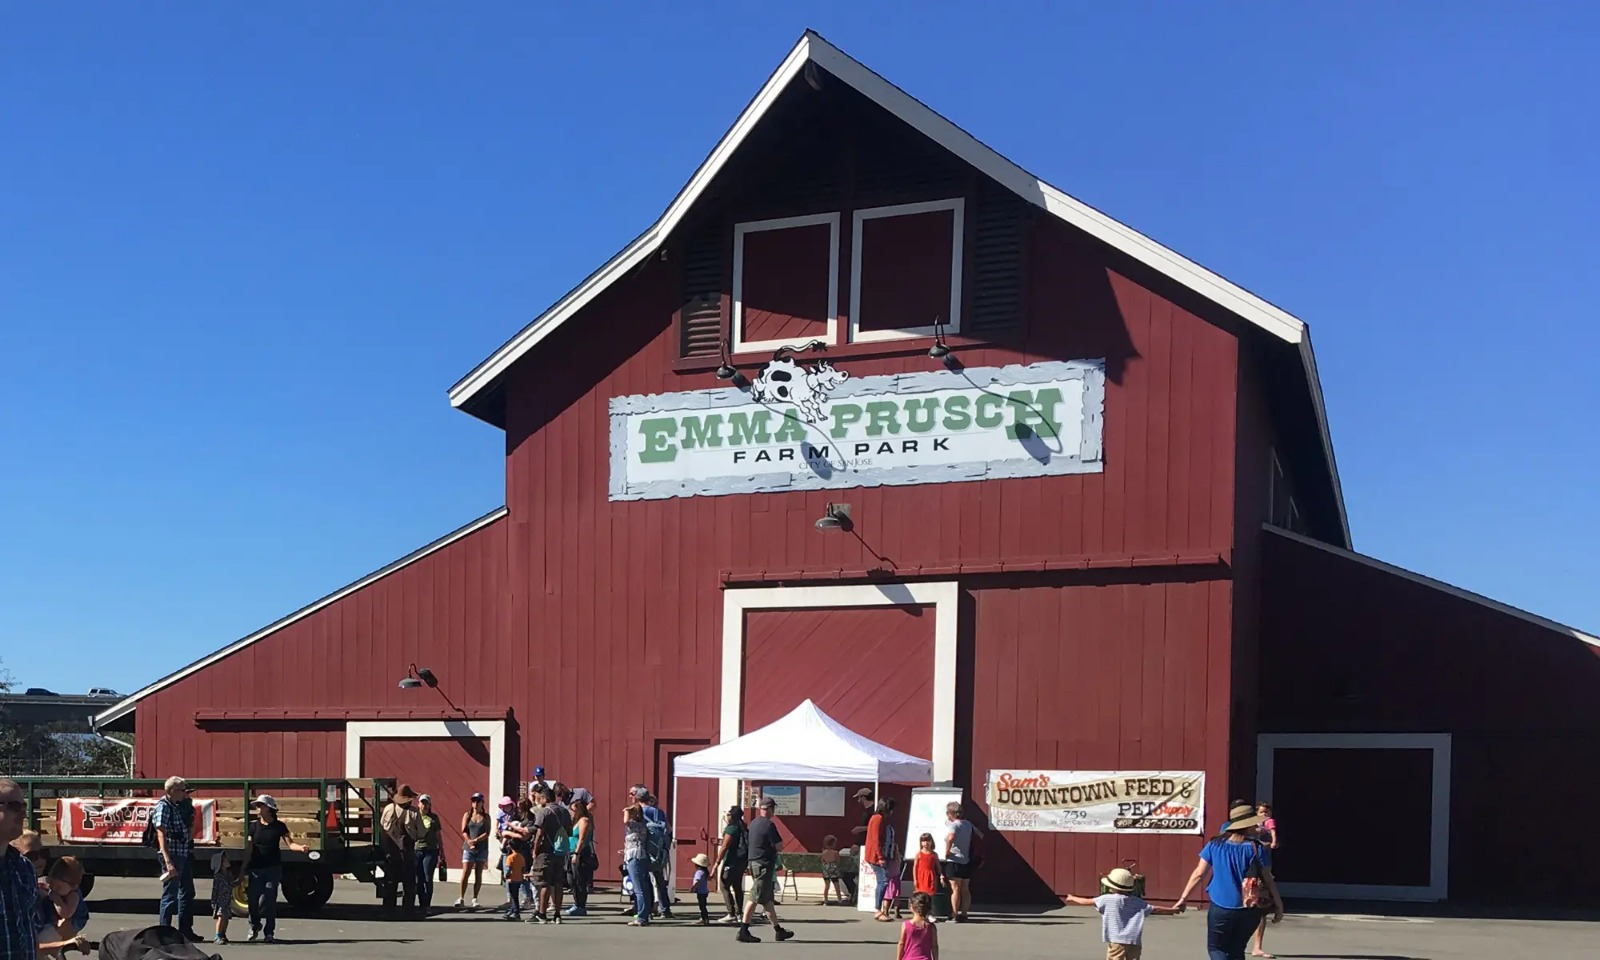
\includegraphics[width=0.8\textwidth]{assets/emma_prusch_farm.png}
  \caption{Emma Prusch Farm Park in San Jose}
  \label{fig:emma_prusch_farm}
  \cite{cruz2024peninsula}
\end{figure}

\subsection{Foothill Community Health Center}

Foothill Community Health Center, serving Evergreen and beyond, plays a critical role in providing accessible healthcare—an essential factor in ensuring community safety and well-being. Immigrants, low-income families, and undocumented residents rely on clinics like these for preventive care, vaccinations, and treatment of work-related injuries and illnesses. The center’s existence speaks to the broader struggle to establish equitable healthcare systems that address the social determinants of health.

By providing culturally competent care and language services, Foothill Community Health Center empowers patients who might otherwise hesitate to seek treatment due to discrimination or financial barriers. Amid national debates over healthcare access, places like this stand as testaments to community resilience and advocacy. They underscore that health and safety are not merely individual concerns but collective responsibilities intertwined with labor conditions, environmental quality, and cultural inclusion.

\begin{figure}[h]
  \centering
  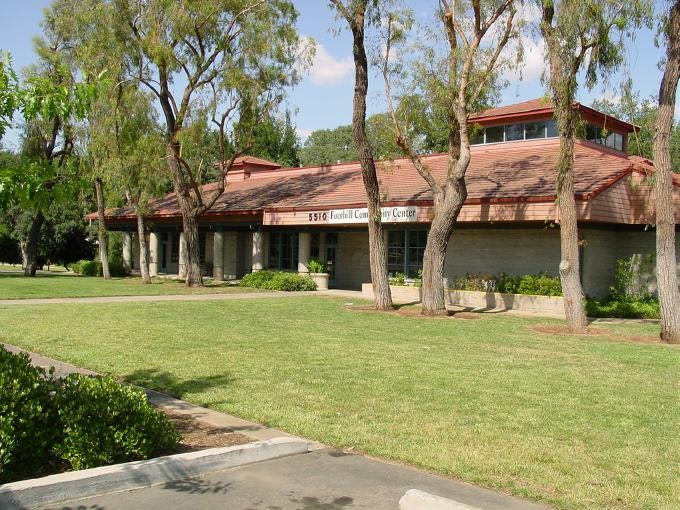
\includegraphics[width=0.8\textwidth]{assets/foothill_center.png}
  \caption{Foothill Community Health Center in San Jose}
  \label{fig:foothill_center}
  \cite{a2017foothill}
\end{figure}

\section{Conclusion}

Standing at the crossroads of past and present, Evergreen’s narrative reveals that the struggles and successes of work and health are deeply interconnected. The orchards and fields that once symbolized prosperity also signified backbreaking labor and hazardous working conditions for immigrant communities. Over time, as the economy shifted toward services, education, and technology, new forms of labor evolved. Yet workers continue to face issues of fair compensation, security, and dignity.

Our tour has showcased how community institutions—from religious centers to healthcare clinics—play crucial roles in fostering safer, healthier lives. These sites illuminate the complexities of immigrant experiences, where language, race, culture, and gender intersect with economic pressures and systemic inequalities. In spaces like Evergreen Valley College and Foothill Community Health Center, we see how education and healthcare challenge entrenched disparities. Similarly, places like Emma Prusch Farm Park and Montgomery Hill Park remind us that history is neither static nor erased; it endures in the very landscapes we inhabit.

By visiting these sites, we understand that health and safety are not guaranteed by suburban comfort alone. They demand vigilance, collective action, and empathy. Evergreen’s story compels us to recognize how local experiences fit into larger national and global patterns. As we depart, we carry with us a deeper awareness: the well-being of any community depends on remembering the past, confronting injustice, and working collaboratively toward a more equitable future.

\bibliographystyle{apalike}
\bibliography{references}

\end{document}
